%Created with command:
%"/home/josh/Teaching/trunk/Utilities/makeexam" "Final Exam" "Please complete each problem.  Show all of your work even if you cannot obtain the correct answer.  You may use only two sheets of letter sized paper for assistance." "../NumberSystems/Assessments/convert_hex_oct_bin_ex.tex" "../NumberSystems/Assessments/twos_complement_ex.tex" "../NumberSystems/Assessments/twos_complement_arithmetic_ex.tex" "../CMOSCircuits/Assessments/cmos_OR_gate_design.tex" "../CombinationalCircuits/Assessments/kmaps_ex.tex" "../VHDL/Assessments/process.tex" "../Decoders/Assessments/2to4decoder.tex" "../XOR/Assessments/memory_parity_extended.tex" "../Muxes/Assessments/74x138_demux.tex" "../LatchesAndFlipFlops/Assessments/latch_flip-flop.tex" "../LatchesAndFlipFlops/Assessments/d_flip-flop_clock.tex" "../StateMachines/Assessments/state_machine_excitation.tex" "../Counters/Assessments/free_running.tex" "../Memory/Assessments/ram_size.tex" "../Memory/Assessments/dram_cell.tex" "../Memory/Assessments/sram_implementation.tex" "../Memory/Assessments/rom_types.tex" "../Memory/Assessments/rom_structure_missing_parts.tex"
\documentclass{article}
\usepackage[T1]{fontenc}
\usepackage{arev}
\usepackage{longtable}
\usepackage[hmargin=2cm,vmargin=2cm]{geometry}
\usepackage{graphicx}
\usepackage{listings}
\setlength{\parindent}{0pt}
\usepackage{fancyhdr}
\pagestyle{fancy}
\renewcommand{\headrulewidth}{0pt}
\fancyhead[LO,LE]{ELEE204}
\fancyhead[CO,CE]{Digital Logic Design}
\fancyhead[RO,RE]{J. Peterson S09}
\cfoot{\thepage}
\title{Final Exam}
\date{}
\begin{document}
\maketitle
\thispagestyle{fancy}
Please complete each problem.  Show all of your work, even if you cannot obtain the correct answer.  You may use only two sheets of letter sized paper for assistance. (80 points total)
\begin{longtable}[l]{rp{17cm}}
%file: ../NumberSystems/Assessments/convert_hex_oct_bin_ex.tex
1.&\begin{minipage}[t]{\linewidth}(4 pt) Perform the following number system conversions. \\
\\
(a) $00101011_2 = ?_{16}$ \\
(b) $00010011_2 = ?_8$ \\
(c) $163_{16} = ?_8$ \\
(d) $\textrm{AFDB} = ?_2$ \\

\vspace{4cm}
\end{minipage}\\
\medskip
%file: ../NumberSystems/Assessments/twos_complement_ex.tex
2.&\begin{minipage}[t]{\linewidth}(2 pt) Find the eight bit two's complement representation of each of the following numbers. \\
\\
(a) $-10$\\
(b) $-36$

\vspace{4cm}
\end{minipage}\\
\medskip
%file: ../NumberSystems/Assessments/twos_complement_arithmetic_ex.tex
3.&\begin{minipage}[t]{\linewidth}(3 pt) Perform the following binary arithmetic using the four bit two's complement representation, showing all carries.  For each case, determine if overflow occurs. If it does, state why it occurs.
\\
\\
$5 + -1$\\

\vspace{4cm}
\end{minipage}\\
\medskip
%file: ../CMOSCircuits/Assessments/cmos_OR_gate_design.tex
4.&\begin{minipage}[t]{\linewidth}(4 pt) Write the function table and draw the circuit diagram for a two input CMOS OR gate.  Note that this gate should use six transistors.\\ \\

\vspace{12cm
}
\end{minipage}\\
\medskip
%file: ../CombinationalCircuits/Assessments/kmaps_ex.tex
5.&\begin{minipage}[t]{\linewidth}(3 pt) Use Karnaugh maps to find a minimal sum of products represention of the following logic function.\\ \\
$F=\prod_{W,X,Y,Z}(6,7,8,9,10,11,12,13,14)$\\

\vspace{12cm
}
\end{minipage}\\
\medskip
%file: ../VHDL/Assessments/process.tex
6.&\begin{minipage}[t]{\linewidth}(2 pt) Briefly describe the role of the sensitivity list in the VHDL process statement.

\vspace{6cm
}
\end{minipage}\\
\medskip
%file: ../Decoders/Assessments/2to4decoder.tex
7.&\begin{minipage}[t]{\linewidth}(10 pt) Using the following logic circuit (a) write a logic function for each output (Y0, Y1, Y2, and Y3) and (b) determine which common component this logic circuit represents.\\
\begin{center}
  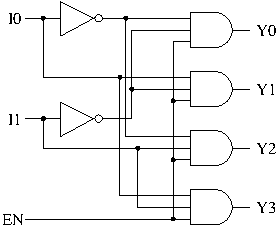
\includegraphics{../Decoders/Assessments/2to4BinaryDecoderLogic} \\
\end{center}

\vspace{8cm
}
\end{minipage}\\
\medskip
%file: ../XOR/Assessments/memory_parity_extended.tex
8.&\begin{minipage}[t]{\linewidth}(8 pt) You have been asked to extend the memory parity circuit to work with a 16 bit data bus.  Given the following schematic diagram, correctly connect the two areas in the dotted lines - the ERROR signal circuit and the PIN input to the memory.  You may need to use some additional logic gates.
\begin{center}
  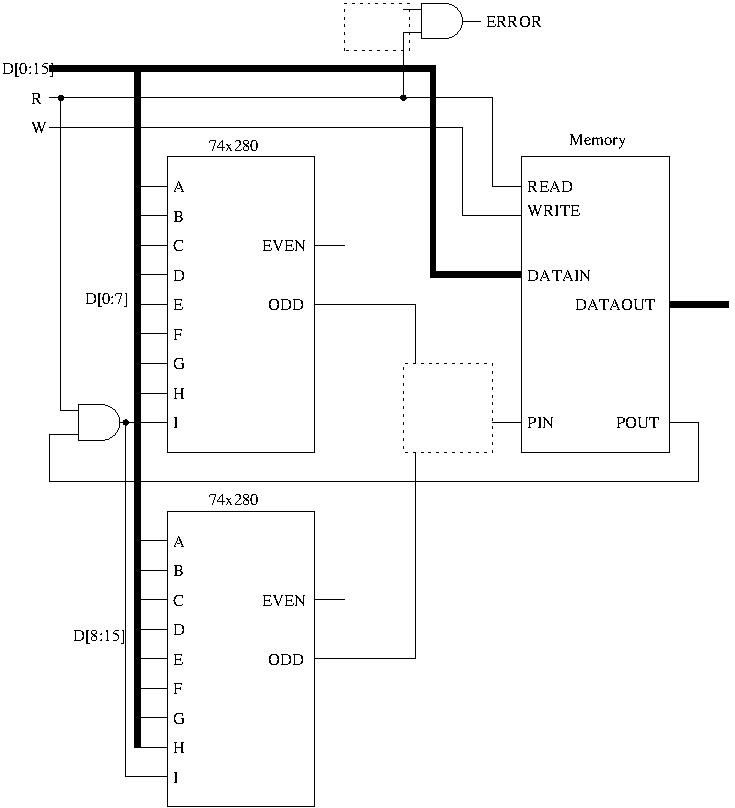
\includegraphics[scale=0.5]{../XOR/Assessments/MemoryCircuitParityExtended}
\end{center}

\vspace{6cm
}
\end{minipage}\\
\medskip
%file: ../Muxes/Assessments/74x138_demux.tex
9.&\begin{minipage}[t]{\linewidth}(4 pt) Using input signals SRC\_L, SEL0, SEL1, and SEL2, configure the inputs of the 74x128 decoder below to cause it to behave as a 1-bit demultiplexer.\\ \\
\begin{center}
  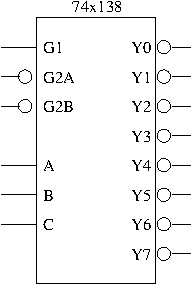
\includegraphics{../Muxes/Assessments/74x138Schematic}
\end{center}

\vspace{4cm
}
\end{minipage}\\
\medskip
%file: ../LatchesAndFlipFlops/Assessments/latch_flip-flop.tex
10.&\begin{minipage}[t]{\linewidth}(2 pt) Briefly explain the key difference between a latch and a flip-flop. \\

\vspace{4cm
}
\end{minipage}\\
\medskip
%file: ../LatchesAndFlipFlops/Assessments/d_flip-flop_clock.tex
11.&\begin{minipage}[t]{\linewidth}(4 pt) The following figure is a partial implementation of a D flip-flop using two D latches.  Correctly connect the clock input (CLK) within the circuit.  Note that you may need to use one or more logic gates to complete this problem. \\ \\
\begin{center}
  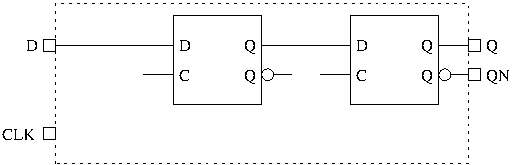
\includegraphics{../LatchesAndFlipFlops/Assessments/DFlipFlopLogicNoClock}
\end{center}

\vspace{8cm
}
\end{minipage}\\
\medskip
%file: ../StateMachines/Assessments/state_machine_excitation.tex
12.&\begin{minipage}[t]{\linewidth}(6 pt) Write the excitation equations for the following state machine.
\begin{center}
  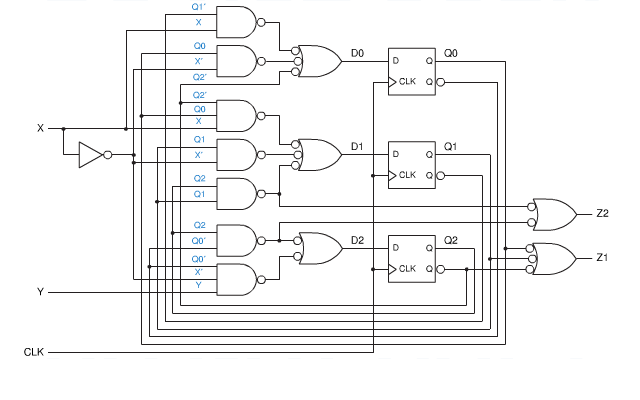
\includegraphics[scale=0.7]{../StateMachines/Assessments/Wakerly_7_43}
\end{center}

\vspace{8cm
}
\end{minipage}\\
\medskip
%file: ../Counters/Assessments/free_running.tex
13.&\begin{minipage}[t]{\linewidth}(6 pt) Configure the 74x163 counter below to be a free running counter. \\ \\
\begin{center}
  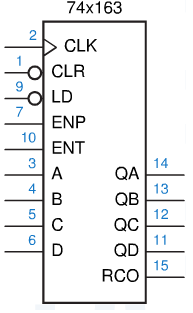
\includegraphics[scale=0.5]{../Counters/Assessments/74x163Schematic}
\end{center}

\vspace{12cm
}
\end{minipage}\\
\medskip
%file: ../Memory/Assessments/ram_size.tex
14.&\begin{minipage}[t]{\linewidth}(2 pt) How many bits of data can a RAM with 4 address bits and 16 data bits store?\\ \\

\vspace{4cm
}
\end{minipage}\\
\medskip
%file: ../Memory/Assessments/dram_cell.tex
15.&\begin{minipage}[t]{\linewidth}(4 pt) Given the following one bit DRAM cell, what voltage levels would you place on the word line and the bit line to write a value of zero to the bit stored?\\ \\
\begin{center}
  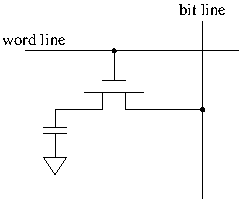
\includegraphics{../Memory/Assessments/DRAMCell}
\end{center}

\vspace{6cm
}
\end{minipage}\\
\medskip
%file: ../Memory/Assessments/sram_implementation.tex
16.&\begin{minipage}[t]{\linewidth}(2 pt) To implement a single bit using SRAM, would you use a D latch or a D flip-flop?\\ \\

\vspace{4cm
}
\end{minipage}\\
\medskip
%file: ../Memory/Assessments/rom_types.tex
17.&\begin{minipage}[t]{\linewidth}(4 pt) Briefly decribe the difference between EEPROM and flash EEPROM.\\ \\

\vspace{4cm
}
\end{minipage}\\
\medskip
%file: ../Memory/Assessments/rom_structure_missing_parts.tex
18.&\begin{minipage}[t]{\linewidth}(10 pt) The following diagram of a ROM with 6 address inputs and 1 data output is missing two standard combinational logic components.  Correctly complete the diagram by drawing and connecting the two components.\\ \\
\begin{center}
  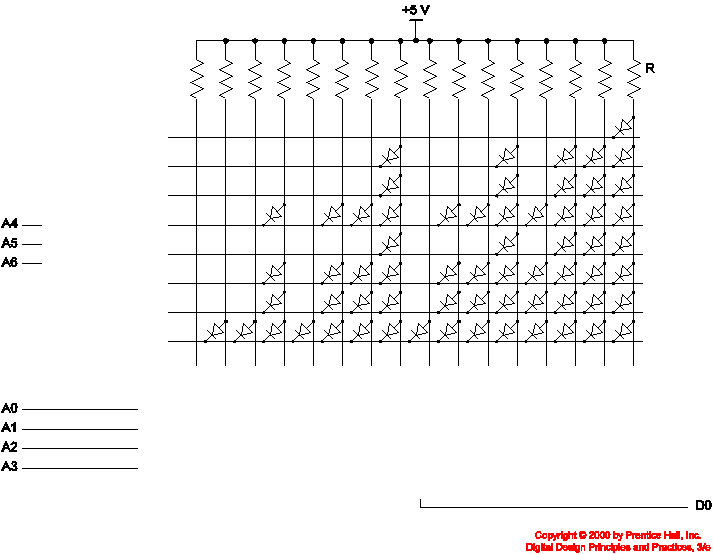
\includegraphics[scale=0.4]{../Memory/Assessments/ROMStructureMissingParts}
\end{center}

\vspace{4cm
}
\end{minipage}\\
\medskip
\end{longtable}
\end{document}
